\documentclass[11pt,a4paper]{article}

\usepackage[margin=0.8in]{geometry}
\usepackage{graphicx}
\usepackage{amsmath,amssymb}
\usepackage{booktabs}
\usepackage{float}
\usepackage{microtype}
\usepackage[hidelinks]{hyperref}
\usepackage{array}
\usepackage{xcolor}
\newcommand{\TBD}[1]{\textcolor{red}{\textbf{#1}}}  % numbers still to be filled in (shown in red)

\title{Large Language Models\\
Homework 1}
\author{Chia-Hsuan Hsu \quad Student ID: 315511079}
\date{Fall 2026}

\begin{document}

\maketitle

% ============================================================
% Problem 1
% ============================================================

\section{N-Gram, RNN, and LSTM Models for Language Identification}

\subsection{Setup}

The course-provided splits are used without modification: 1,120
training, 140 validation, and 140 test texts per language (5,600 / 700 /
700 in total). A shared character vocabulary of size $|V|=129$ is built
from \texttt{train.csv} only, including the special tokens
\texttt{<PAD>}, \texttt{<UNK>}, \texttt{<BOS>}, and \texttt{<EOS>}.
Characters that never occur in the training data are mapped to
\texttt{<UNK>}. All models use the same vocabulary and the same
special-token policy: \texttt{<BOS>} and \texttt{<PAD>} are never
prediction targets, while \texttt{<EOS>} is. Every text is assigned to
the language whose model gives the lowest perplexity,
\[
\hat{l}=\arg\min_{l\in\mathcal{L}}\mathrm{PPL}(x\mid l),
\]
and all validation and test perplexities are corpus-level: the total
negative log-likelihood under the ground-truth language model divided by
the total number of prediction targets. Per-text perplexities are never
averaged.

% ------------------------------------------------------------

\subsection{Character-Level Bigram and Trigram Models}

For each language, bigram and trigram counts are collected from its
training texts and smoothed with Add-$\alpha$ ($\alpha=1$):
\[
p(c_t\mid c_{t-1},l)=\frac{C_l(c_{t-1},c_t)+\alpha}{C_l(c_{t-1})+\alpha|V|},\qquad
p(c_t\mid c_{t-2},c_{t-1},l)=\frac{C_l(c_{t-2},c_{t-1},c_t)+\alpha}{C_l(c_{t-2},c_{t-1})+\alpha|V|}.
\]
Each text is left-padded with $n-1$ \texttt{<BOS>} tokens. As a result,
the first character is also predicted, and both models score exactly the
same targets: every character plus \texttt{<EOS>}.

\begin{table}[H]
    \centering
    \caption{Results of the $n$-gram models.}
    \label{tab:p1-ngram}
    \begin{tabular}{lcccccc}
        \toprule
        Model & Val PPL & Test PPL & Accuracy & Macro-F1 & Build time (s) & Inference time (s)\\
        \midrule
        Bigram  & 11.4373 & 11.3264 & 0.9729 & 0.9727 & 1.913 & 0.166\\
        Trigram & \textbf{9.7008} & \textbf{9.4022} & \textbf{0.9871} & \textbf{0.9871} & 2.120 & 0.184\\
        \bottomrule
    \end{tabular}
\end{table}

\begin{figure}[H]
    \centering
    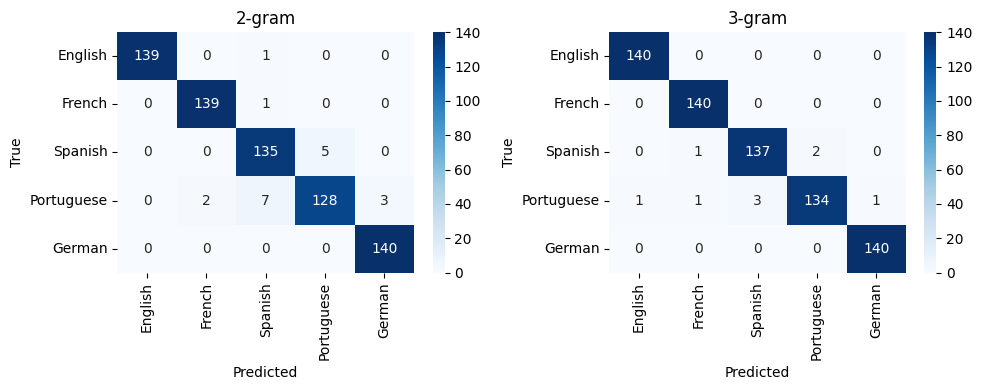
\includegraphics[width=\linewidth]{fig1-part1.png}
    \caption{Test confusion matrices of the bigram (left) and trigram
    (right) models.}
    \label{fig:p1-ngram-cm}
\end{figure}

\paragraph{Results.}
The trigram model is better than the bigram model on every metric.
Its validation perplexity is 9.70 instead of 11.44, and its test
accuracy is 0.9871 instead of 0.9729. With two characters of context,
the trigram model can capture language-specific patterns such as
\emph{-ção} (Portuguese) versus \emph{-ción} (Spanish), or \emph{sch}
and \emph{th}.

\paragraph{Cost.}
Both models are built in about 2\,s on a CPU and need very little
memory. The peak memory during construction is 0.42\,MB for the bigram
and 2.64\,MB for the trigram. The trigram uses more memory because the
number of possible contexts grows from $|V|$ to $|V|^2$. Classifying all
700 test texts takes less than 0.2\,s.

\paragraph{Error analysis.}
As Figure~\ref{fig:p1-ngram-cm} shows, almost all errors involve
Portuguese or Spanish. The bigram model misclassifies 12 Portuguese texts
(7 as Spanish) and 5 Spanish texts (as Portuguese). The trigram model
reduces this to 6 Portuguese and 3 Spanish errors. Representative
errors are mostly very short or contain little language-specific
evidence:
\begin{itemize}
    \item ``\texttt{4.800 --}'' (Portuguese, 8 characters), predicted as
          German by both $n$-gram models. It contains no letters at all.
    \item ``\emph{Decidimos,}'' (Portuguese), predicted as Spanish. The
          word is spelled identically in both languages.
    \item ``\emph{to protect us}'' (English), predicted as Spanish, and
          ``\emph{un monde de murs,}'' (French), predicted as Spanish.
    \item ``\emph{Ándale! Ándale!}'' in the Portuguese test set,
          predicted as German. This is a Spanish expression quoted inside
          a Portuguese talk.
\end{itemize}

% ------------------------------------------------------------

\subsection{Character-Level RNN Language Models}

Five character-level language models are trained, one per language,
using the suggested settings: embedding dimension 128, hidden dimension
128, 2 layers, Adam with learning rate 0.001, 10 epochs, batch size 32,
and cross-entropy loss. The input is \texttt{<BOS>} followed by the
characters of the text. The target is the next character, ending with
\texttt{<EOS>}, and padded positions are ignored in the loss. For each
language, the checkpoint with the lowest validation perplexity is kept.

\begin{figure}[H]
    \centering
    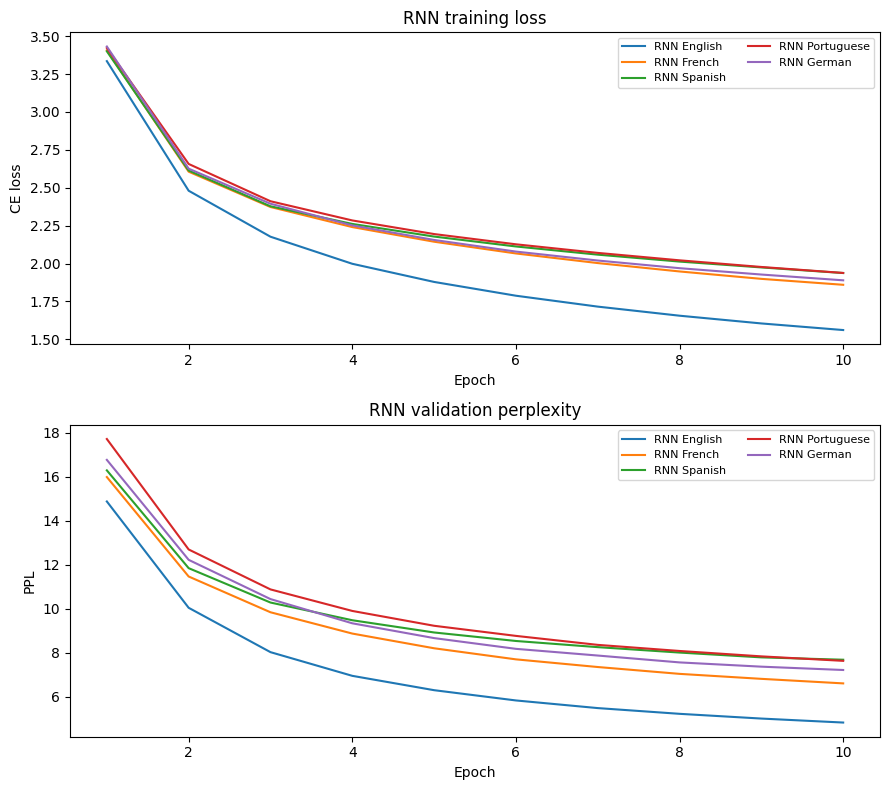
\includegraphics[width=0.8\linewidth]{fig2-part1.png}
    \caption{RNN training loss (top) and validation perplexity (bottom)
    for the five languages.}
    \label{fig:p1-rnn-curves}
\end{figure}

As Figure~\ref{fig:p1-rnn-curves} shows, the training loss decreases
steadily for all languages, falling from about 3.4 to between 1.56 and
1.94. The validation perplexity follows the same trend. Both curves are
still decreasing at epoch 10, so the last epoch is selected for every
language and no overfitting is observed. The best per-language
validation perplexities are:
\begin{itemize}
    \item English: 4.83
    \item French: 6.60
    \item German: 7.21
    \item Portuguese: 7.63
    \item Spanish: 7.68
\end{itemize}
English is the easiest to model because its spelling uses almost no
diacritics.

\begin{table}[H]
    \centering
    \caption{Test confusion matrix of the RNN models (rows: true language,
    columns: predicted language).}
    \label{tab:p1-rnn-cm}
    \begin{tabular}{lccccc}
        \toprule
        True $\backslash$ Pred & English & French & Spanish & Portuguese & German\\
        \midrule
        English    & 139 & 1   & 0   & 0   & 0\\
        French     & 0   & 140 & 0   & 0   & 0\\
        Spanish    & 0   & 1   & 136 & 3   & 0\\
        Portuguese & 0   & 2   & 2   & 135 & 1\\
        German     & 0   & 0   & 0   & 0   & 140\\
        \bottomrule
    \end{tabular}
\end{table}

\paragraph{Results.}
On \texttt{test.csv} the RNN models obtain:
\begin{itemize}
    \item Accuracy: 0.9857
    \item Macro-F1: 0.9857
    \item Corpus-level test perplexity: 5.7054 (validation: 5.8937)
\end{itemize}

\paragraph{Cost.}
Training the five models takes 6.4\,s in total on the GPU, with a peak
GPU memory of 391.7\,MB. Inference over the test set takes 4.1\,s
because every text must be passed through all five models.

\paragraph{Correct and incorrect predictions.}
Even very short texts are identified correctly when they contain
language-specific function words or diacritics. Examples include
``\emph{Il est si}'' (French, 9 characters), ``\emph{é preciosa,}''
(Portuguese), and ``\emph{Y escalamos}'' and ``\emph{Son una red}''
(Spanish). As Table~\ref{tab:p1-rnn-cm} shows, the 10 errors are
concentrated on Spanish and Portuguese. These are short phrases made of
words that are spelled the same or almost the same in both languages,
which leaves too little evidence to separate them.

% ------------------------------------------------------------

\subsection{Character-Level LSTM Language Models}

The LSTM models use exactly the same split, vocabulary, loss, optimiser,
and hyperparameters as the RNN models. The only change is that the RNN
layers are replaced with LSTM layers.

\begin{figure}[H]
    \centering
    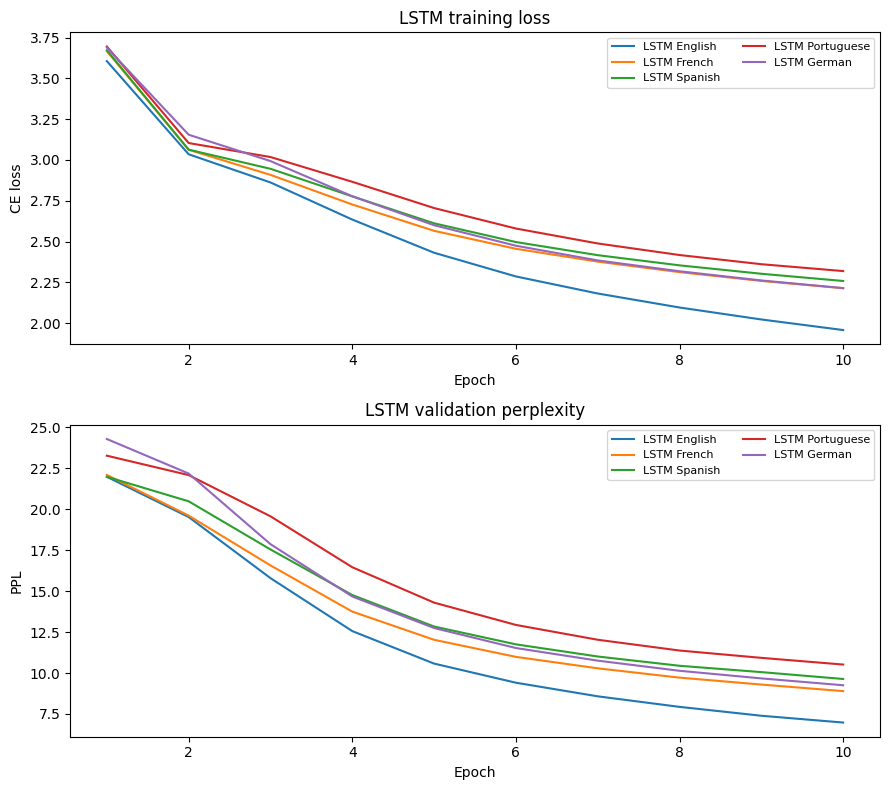
\includegraphics[width=0.8\linewidth]{fig5-part1.png}
    \caption{LSTM training loss (top) and validation perplexity (bottom)
    for the five languages.}
    \label{fig:p1-lstm-curves}
\end{figure}

\begin{figure}[H]
    \centering
    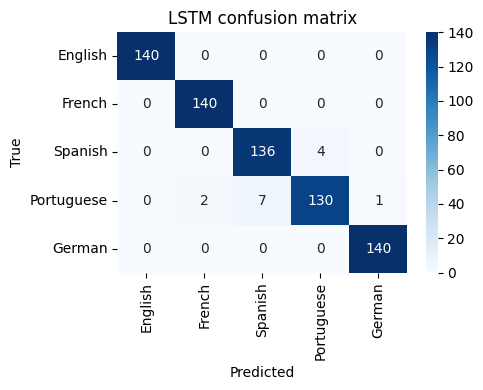
\includegraphics[width=0.5\linewidth]{fig3-part1.png}
    \caption{Test confusion matrix of the LSTM models.}
    \label{fig:p1-lstm-cm}
\end{figure}

\paragraph{Learning curves.}
The LSTM curves (Figure~\ref{fig:p1-lstm-curves}) also decrease
monotonically, but they start higher and converge more slowly than the
RNN curves. After 10 epochs, the training loss is between 1.96 and 2.32,
and the best validation perplexities are:
\begin{itemize}
    \item English: 6.98
    \item French: 8.90
    \item German: 9.25
    \item Spanish: 9.64
    \item Portuguese: 10.52
\end{itemize}
These are all higher than the RNN values. An LSTM has four gates per
step and therefore about four times as many recurrent parameters, so the
same 10-epoch budget leaves it further from convergence.

\paragraph{Results.}
On \texttt{test.csv} the LSTM models obtain:
\begin{itemize}
    \item Accuracy: 0.9800
    \item Macro-F1: 0.9799
    \item Corpus-level test perplexity: 7.9834 (validation: 8.1334)
\end{itemize}

\paragraph{Cost.}
Training takes 9.0\,s, with a peak GPU memory of 563.3\,MB, and
inference over the test set takes 5.1\,s. Both are higher than for the
RNN because of the larger recurrent cell.

\paragraph{Correct and incorrect predictions.}
Short texts such as ``\emph{Il est si}'', ``\emph{Se comunican}'', and
``\emph{as intuições}'' are identified correctly. As
Figure~\ref{fig:p1-lstm-cm} shows, all 14 errors are Spanish or
Portuguese texts: 7 Portuguese texts are predicted as Spanish, 4 Spanish
texts as Portuguese, and the remaining 3 Portuguese texts as French or
German.

% ------------------------------------------------------------

\subsection{Comparison and Discussion}

\begin{table}[H]
    \centering
    \caption{Comparison of the four model families on \texttt{test.csv}.}
    \label{tab:p1-summary}
    \small
    \begin{tabular}{lccccccc}
        \toprule
        Model & Val PPL & Test PPL & Accuracy & Macro-F1 & Train (s) & Inference (s) & Peak memory\\
        \midrule
        Bigram  & 11.44 & 11.33 & 0.9729 & 0.9727 & 1.91 & 0.17 & 0.42 MB (CPU)\\
        Trigram & 9.70  & 9.40  & \textbf{0.9871} & \textbf{0.9871} & 2.12 & 0.18 & 2.64 MB (CPU)\\
        RNN     & \textbf{5.89} & \textbf{5.71} & 0.9857 & 0.9857 & 6.42 & 4.08 & 391.7 MB (GPU)\\
        LSTM    & 8.13  & 7.98  & 0.9800 & 0.9799 & 9.01 & 5.13 & 563.3 MB (GPU)\\
        \bottomrule
    \end{tabular}
\end{table}

\begin{figure}[H]
    \centering
    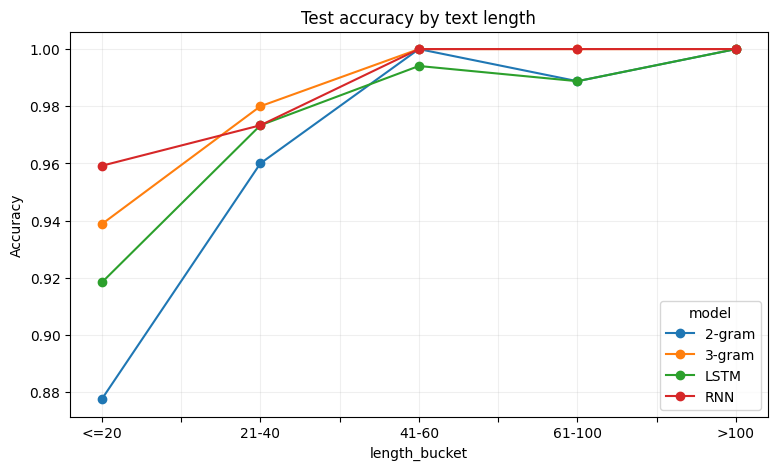
\includegraphics[width=0.75\linewidth]{fig4-part1.png}
    \caption{Test accuracy as a function of text length (number of
    characters).}
    \label{fig:p1-length}
\end{figure}

\paragraph{Hardware and computation time.}
The $n$-gram models only need a CPU and a few megabytes of memory. They
are built in about 2\,s and classify the entire test set in under
0.2\,s. The RNN and LSTM models need a GPU, with 392\,MB and 563\,MB of
peak GPU memory respectively. They take longer to train, and their
inference is more than 20 times slower, because every text requires a
sequential forward pass through five neural models.

\paragraph{Does lower perplexity always mean higher accuracy? No.}
The RNN has by far the lowest perplexity (5.71, compared with 9.40 for
the trigram), yet the trigram achieves the highest accuracy (0.9871
versus 0.9857). Likewise, the LSTM has lower perplexity than the trigram
but lower accuracy. Corpus perplexity measures how well the correct
language model predicts its own texts, averaged over all characters.
Identification, however, depends only on the relative ranking of the
five models for each individual text. A model can model long texts very
well and still rank the wrong language first on a few short, ambiguous
texts. Lower perplexity therefore tends to help, but it does not
guarantee better identification accuracy.

\paragraph{Most frequently confused languages.}
Summed over all four models, the most frequent directed confusions are:
\begin{itemize}
    \item Portuguese $\rightarrow$ Spanish: 19
    \item Spanish $\rightarrow$ Portuguese: 14
    \item Portuguese $\rightarrow$ French: 7
    \item Portuguese $\rightarrow$ German: 6
\end{itemize}
Spanish and Portuguese are by far the most confusable pair, because they
share most of their vocabulary and character patterns. English, French,
and German are almost never confused with one another.

\paragraph{Are shorter texts harder?}
Yes. As Figure~\ref{fig:p1-length} shows, every model performs worst on
the shortest texts (at most 20 characters, 49 test samples). In that
group, accuracy is 0.878 for the bigram, 0.918 for the LSTM, 0.939 for
the trigram, and 0.959 for the RNN. Accuracy then rises with length:
\begin{itemize}
    \item 21--40 characters: 0.960--0.980
    \item 41 characters or more: 0.989--1.000
\end{itemize}
Short texts provide only a few characters of evidence, and a single
number, name, or shared word can dominate the score. Longer texts
accumulate enough language-specific patterns to be classified almost
perfectly. The RNN is the most robust model on short texts, while the
bigram is the least robust.



% ============================================================
% Problem 2
% ============================================================

\section{Self-Attention Layer for Semantic Similarity Scoring}

\subsection{Implementation Rules and Model Design}

The provided notebook \texttt{atten.ipynb} was used as the starting
point. Following the course announcement, only the code inside the
\texttt{TODO} and \texttt{TODO (Optional)} blocks was changed. The data
loading, vocabulary, dataset, training loop, evaluation, and submission
code are the provided versions. Additional cells were appended only to
run the experiments in (c) and (d) and the ensemble in (e). These cells
call the provided functions and do not modify them. The ensemble is
placed in a separate code cell, as permitted by the TA.

Each example is converted into a single token sequence
\[
z=\texttt{<context>}\ \text{context}\ \texttt{<sep>}\ \text{anchor}\ \texttt{<sep>}\ \text{target},
\]
using the provided tokenizer and the vocabulary built from
\texttt{train.csv} (vocabulary size 7,749). The fixed settings are
$\texttt{MAX\_LEN}=64$, $d_{\text{model}}=128$, 2 encoder layers,
batch size 64, seed 42, and the MSE training loss. Model selection uses
the epoch with the highest validation Pearson correlation, which the
provided \texttt{train\_model} already does.

\paragraph{Multi-head self-attention (TODO).}
The layer is implemented from scratch, without PyTorch's built-in
multi-head attention module (\texttt{torch.nn.\allowbreak MultiheadAttention}). $Q$, $K$, and $V$ are linear
projections of the input, split into $h$ heads of size $d_k=128/h$.
For each head,
\[
\mathrm{Attn}(Q,K,V)=\mathrm{softmax}\!\left(\frac{QK^\top}{\sqrt{d_k}}+M\right)V,
\]
where $M$ sets the scores of padded key positions to $-10^{9}$. The
heads are concatenated and passed through an output projection.

\paragraph{Encoder layer (TODO).}
Each layer uses post-layer normalisation as in the original Transformer,
\[
x \leftarrow \mathrm{LN}\big(x+\mathrm{Drop}(\mathrm{MHA}(x))\big),\qquad
x \leftarrow \mathrm{LN}\big(x+\mathrm{Drop}(\mathrm{FFN}(x))\big),
\]
with $\mathrm{FFN}=\mathrm{Linear}\rightarrow\mathrm{ReLU}\rightarrow\mathrm{Dropout}\rightarrow\mathrm{Linear}$.
In the tuned model, the layer input is first normalised by an extra
LayerNorm. The provided embedding is initialised from $\mathcal N(0,1)$
and multiplied by $\sqrt{128}\approx11.3$, while the attention output
is of order 1. Without the input normalisation, $x+\mathrm{MHA}(x)$ in
the first layer is dominated by the embedding and the first attention
sub-layer has almost no effect.

\paragraph{Pooling (TODO Optional).}
The anchor and target positions are recovered from \texttt{input\_ids}
alone: $\mathrm{cumsum}(\texttt{input\_ids}=\texttt{<sep>})$ is 0 for
the context, 1 for the anchor, and 2 for the target. From the encoder
output, masked means are taken over the whole sequence ($g$), the anchor
words ($u$), and the target words ($v$). Three strategies were used:
\begin{itemize}
    \item \textbf{mean} (default): masked mean over all tokens.
    \item \textbf{interact} (parameter-free): a 128-dimensional vector
          made of three slices, $g$ (32 dimensions), $u\odot v$ (48), and
          $|u-v|$ (48).
    \item \textbf{mlp}: the full vector $[g,u,v,|u-v|,u\odot v]$ is
          passed through $\mathrm{Linear}(5d\rightarrow d)\rightarrow
          \mathrm{GELU}\rightarrow\mathrm{Dropout}$. Optional extra
          inputs are token-level soft-alignment features
          (ESIM-style; ``am'', ``adf'') and max-pooled anchor/target
          vectors (``umax'', ``vmax''). The projection is created inside
          the pooling TODO block.
\end{itemize}
In every case the output has size $d$, so the provided regression head
$\hat s=\sigma(Wh_{\text{pool}}+b)$ is reused unchanged.

\paragraph{Optimiser and scheduler (TODO).}
AdamW is used with two parameter groups. The token embedding has its own
learning rate (a multiple of the base rate), because its weights are of
order 1 and an Adam step of $10^{-3}$ changes them by only about 0.1\%.
The scheduler is a per-epoch linear warm-up (2 epochs) followed by cosine
decay.

\paragraph{Final setting.}
4 heads, \texttt{mlp} pooling with $[g,u,v,|u-v|,u\odot v]$, input
LayerNorm, dropout 0.1, base learning rate $10^{-3}$ with a $20\times$
embedding learning rate, weight decay 0.01, warm-up + cosine schedule,
and 25 epochs.

% ------------------------------------------------------------

\subsection{(a) Learning Curves with 4 Heads}

Figure~\ref{fig:p2-curves} shows the learning curves of the main 4-head
model (final setting).

\begin{figure}[H]
    \centering
    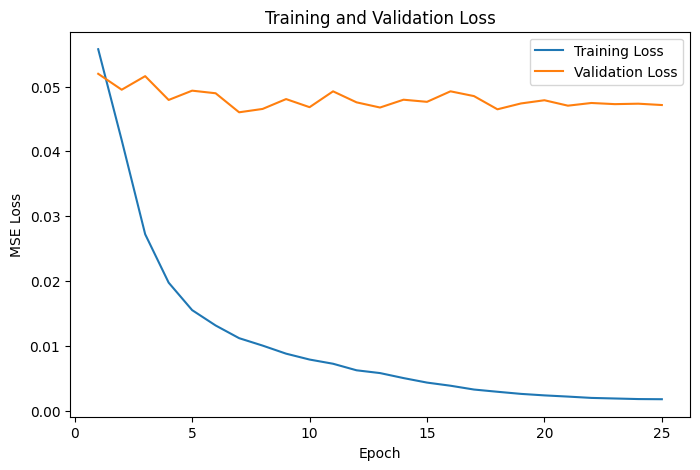
\includegraphics[width=0.49\linewidth]{p2_main_loss.png}\hfill
    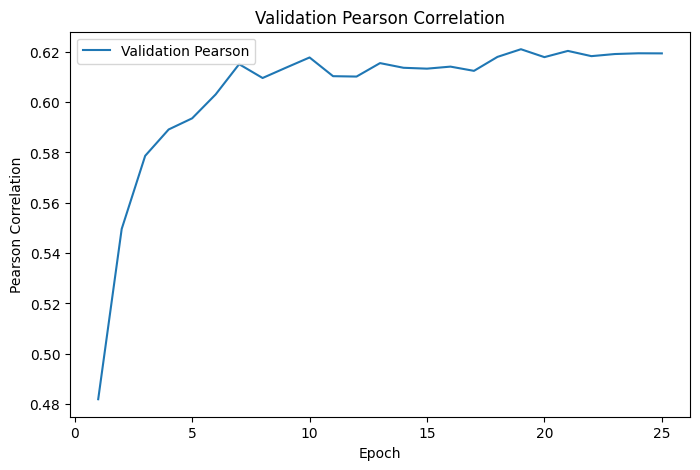
\includegraphics[width=0.49\linewidth]{p2_main_pearson.png}
    \caption{Main model with 4 heads. Left: training and validation MSE
    loss. Right: validation Pearson correlation.}
    \label{fig:p2-curves}
\end{figure}

The training loss falls quickly, from 0.0558 at epoch 1 to 0.0018 at
epoch 25. The validation loss reaches its minimum of 0.0460 at epoch 7
and then stays between 0.046 and 0.049. After a few epochs the model
therefore fits the training set far better than the validation set,
which is clear overfitting. The validation Pearson correlation still
rises after the validation loss stops improving: from 0.4819 at epoch 1
to 0.6151 at epoch 7, reaching its maximum of 0.6210 at epoch 19. The
model keeps improving the ranking of the pairs even when the squared
error no longer decreases. Because the provided \texttt{train\_model}
keeps the checkpoint with the best validation Pearson, the late-epoch
overfitting does not harm the selected model.

% ------------------------------------------------------------

\subsection{(b) Validation Performance}

Using the checkpoint with the best validation Pearson correlation
(epoch 19), the 4-head main model obtains
\[
\text{Pearson}=0.6210,\qquad \text{RMSE}=0.2177,\qquad \text{MSE}=0.0474
\]
on \texttt{val.csv}. For reference, the default baseline with 4 heads
(mean pooling, no scheduler, 10 epochs; D0 in Table~\ref{tab:p2-tuning})
reaches Pearson 0.3173 and RMSE 0.2487.

% ------------------------------------------------------------

\subsection{(c) Effect of the Number of Attention Heads}

The number of heads was set to 1, 4, and 8. The data split, seed,
optimiser, and 10-epoch budget were kept the same, using the default
baseline setting (mean pooling, AdamW with learning rate $10^{-3}$ and
weight decay $10^{-4}$, no scheduler).

\begin{table}[H]
    \centering
    \caption{Validation performance for different numbers of attention heads.}
    \label{tab:p2-heads}
    \begin{tabular}{ccccc}
        \toprule
        Heads & Head dimension & Best val Pearson & Val RMSE & Training time (s)\\
        \midrule
        1 & 128 & \textbf{0.3282} & \textbf{0.2474} & 74.6\\
        4 & 32  & 0.3173 & 0.2487 & 76.2\\
        8 & 16  & 0.2968 & 0.2491 & 76.1\\
        \bottomrule
    \end{tabular}
\end{table}

\begin{figure}[H]
    \centering
    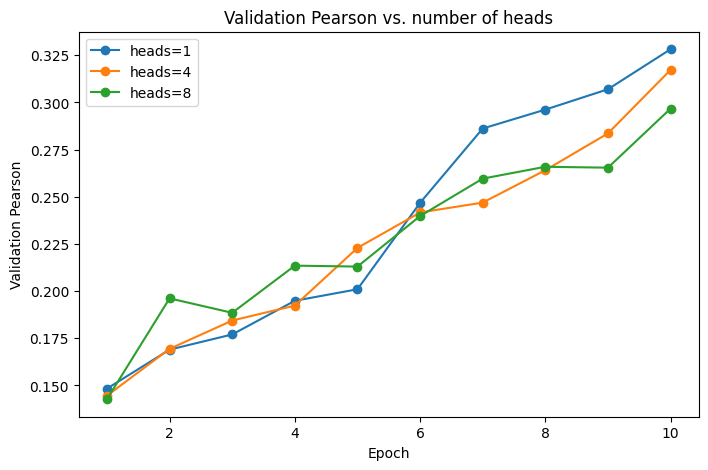
\includegraphics[width=0.7\linewidth]{p2_heads.png}
    \caption{Validation Pearson correlation per epoch for 1, 4, and 8
    attention heads.}
    \label{fig:p2-heads}
\end{figure}

All three settings have the same number of parameters, because the
$Q$, $K$, $V$, and output projections are always $128\times128$. Only
the way the 128-dimensional space is split into heads changes.

As Table~\ref{tab:p2-heads} shows, fewer heads perform slightly better:
1 head reaches 0.3282, 4 heads 0.3173, and 8 heads 0.2968. The RMSE
values are almost identical (0.2474 to 0.2491). The inputs are very
short (about 8 tokens), and the main signal is a word-level match
between the anchor and the target. A single head with 128-dimensional
queries and keys has a richer similarity function. With 8 heads, each
head computes its attention scores in only 16 dimensions, which makes
them noisier. Training time is nearly the same for all three
(74.6--76.2\,s).

The differences are small (0.03 Pearson at most), and all curves are
still rising at epoch 10 (Figure~\ref{fig:p2-heads}). The comparison
therefore mainly reflects how fast each setting converges under the same
budget. The number of heads is not the bottleneck for this task. Much
larger gains come from the changes in (d), so the 4-head setting
required by the assignment is kept for the main model.

% ------------------------------------------------------------

\subsection{(d) Tuning Permitted Settings}

Starting from the baseline D0, each configuration adds one documented
change, using only settings inside the \texttt{TODO} /
\texttt{TODO (Optional)} blocks: hyperparameters, the optimiser, the
scheduler, the pooling strategy, and the inside of the attention and
encoder-layer classes. Every configuration is trained from seed 42.

\begin{table}[H]
    \centering
    \caption{Tuning experiments on \texttt{val.csv}. ``Base'' is the
    configuration the change is applied to.}
    \label{tab:p2-tuning}
    \small
    \begin{tabular}{l l p{0.45\linewidth} ccc}
        \toprule
        ID & Base & Change & Val Pearson & Val RMSE & Best epoch\\
        \midrule
        D0  & --  & Baseline: mean pooling, AdamW (wd $10^{-4}$), no scheduler, 10 epochs & 0.3173 & 0.2487 & 10\\
        D1  & D0  & 25 epochs, 2-epoch warm-up + cosine decay, weight decay 0.01 & 0.4196 & 0.2436 & 25\\
        D2  & D1  & \texttt{interact} pooling (parameter-free) & 0.4871 & 0.2568 & 24\\
        D3  & D2  & Input LayerNorm in each encoder layer & 0.5175 & 0.2540 & 25\\
        D4  & D3  & Relative-position bias in attention & 0.5260 & 0.2505 & 25\\
        D5  & D3  & $10\times$ embedding learning rate & 0.5919 & 0.2267 & 22\\
        D6  & D3  & $30\times$ embedding learning rate & 0.5965 & 0.2249 & 25\\
        D7  & D5  & Relative-position bias & 0.6001 & 0.2249 & 25\\
        D8  & D5  & \texttt{mlp} pooling $[g,u,v,|u-v|,u\odot v]$ & 0.6161 & 0.2310 & 21\\
        D9  & D8  & Dropout $0.2\rightarrow0.1$ & 0.6262 & 0.2143 & 20\\
        D10 & D9  & $20\times$ embedding learning rate (\textbf{final setting}) & 0.6394 & 0.2108 & 14\\
        D11 & D10 & + alignment features (am, adf) & 0.6244 & 0.2103 & 23\\
        D12 & D10 & + max-pooled features (umax, vmax) & \textbf{0.6400} & \textbf{0.2091} & 16\\
        D13 & D10 & + alignment and max-pooled features & 0.6324 & 0.2093 & 16\\
        \bottomrule
    \end{tabular}
\end{table}

\begin{figure}[H]
    \centering
    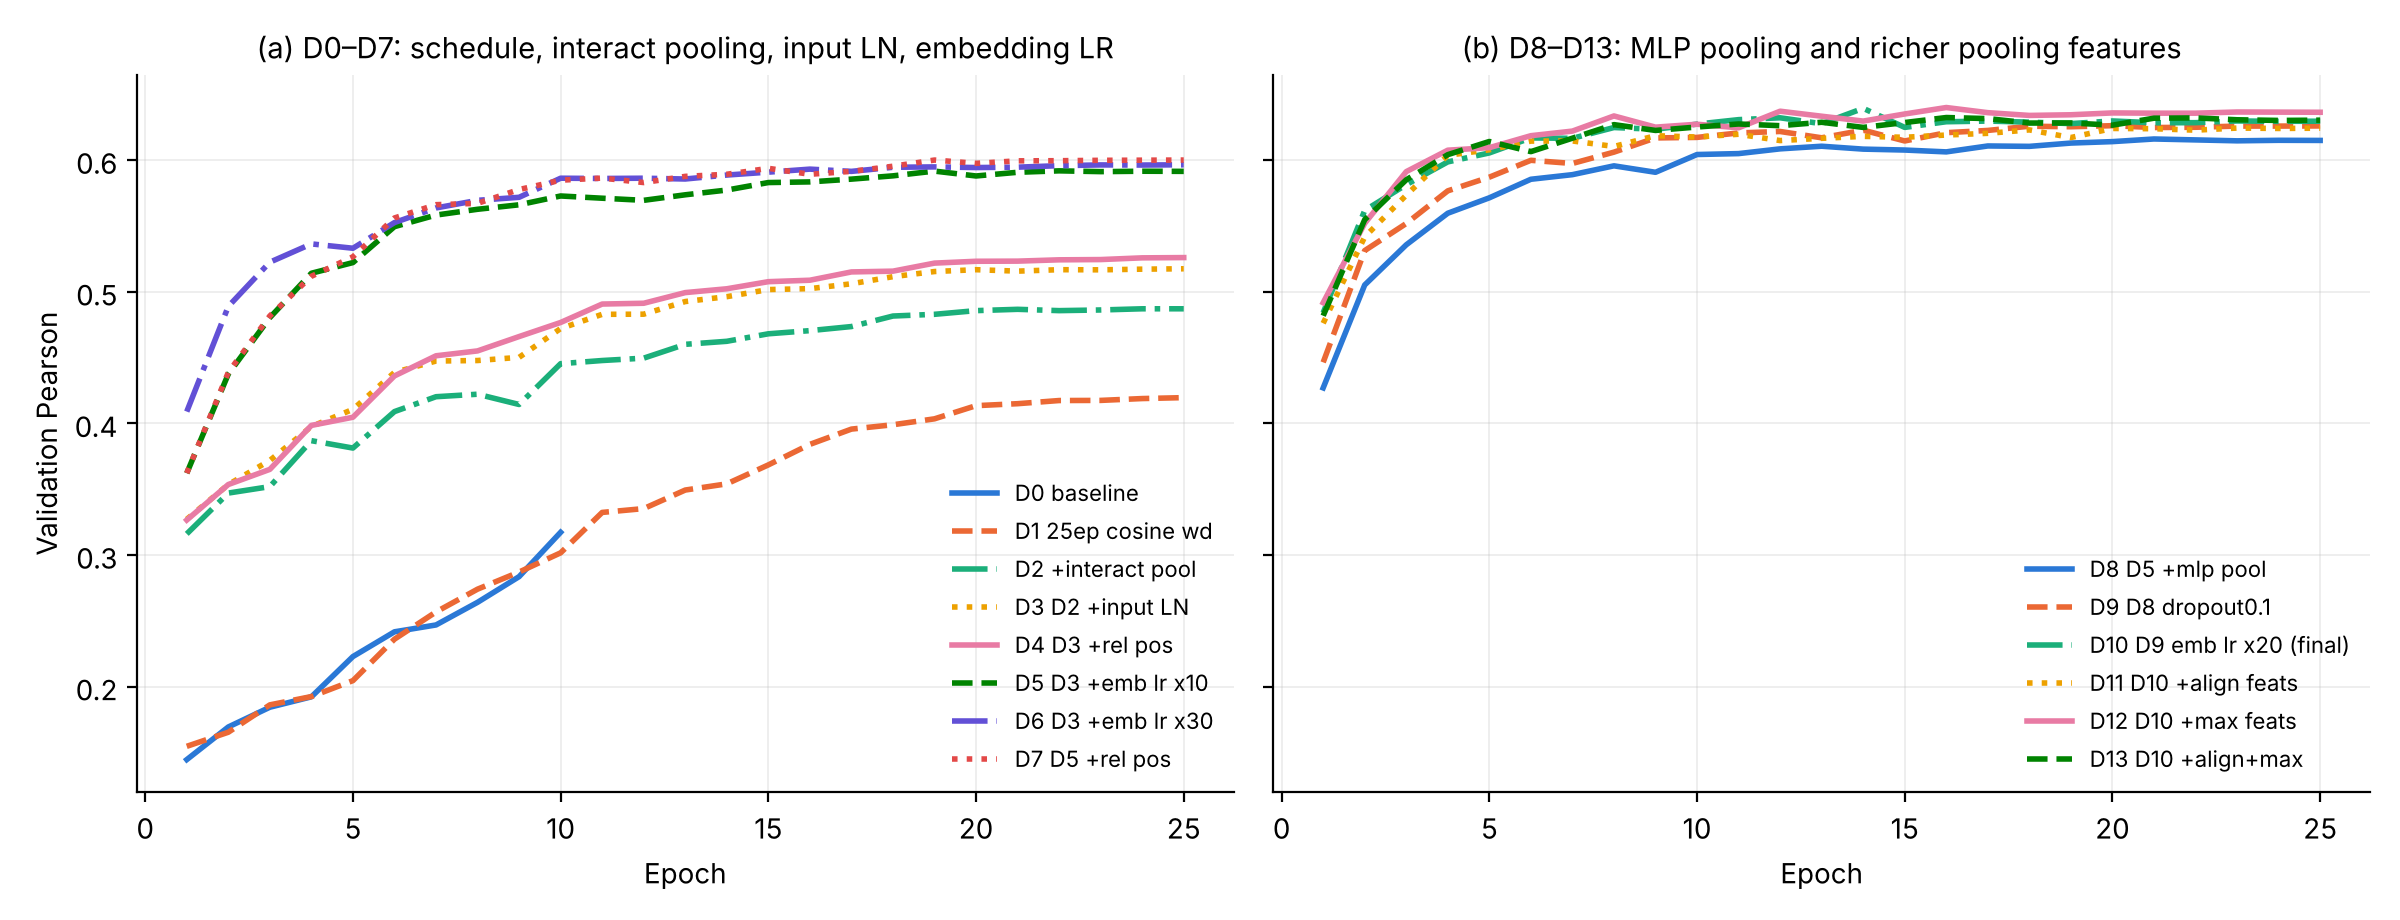
\includegraphics[width=\linewidth]{p2_tuning.png}
    \caption{Validation Pearson correlation per epoch for the tuning
    configurations. (a) D0--D7. (b) D8--D13.}
    \label{fig:p2-tuning}
\end{figure}

\paragraph{D1: longer budget, schedule, and weight decay (+0.102).}
The baseline is still improving at epoch 10. With 25 epochs, a
warm-up + cosine schedule, and stronger weight decay, the validation
Pearson rises to 0.4196. Figure~\ref{fig:p2-tuning}a shows that the D1
curve is still rising at epoch 25, so mean pooling learns slowly.

\paragraph{D2: interaction pooling (+0.068).}
Mean pooling mixes the context, anchor, and target into one vector, so
the regression head cannot tell which phrase a feature comes from. The
parameter-free \texttt{interact} pooling exposes the alignment
$u\odot v$ and the difference $|u-v|$ directly and raises the Pearson
correlation to 0.4871. Its RMSE is slightly higher (0.2568), probably
because the fixed slices change the scale of the features fed to the
linear head. Model selection uses Pearson correlation, so this is
acceptable.

\paragraph{D3--D7: fixing the embedding scale.}
The input LayerNorm (D3) lets the first attention sub-layer contribute
and adds 0.030. The relative-position bias adds little: +0.009 on D3
(D4) and +0.008 on D5 (D7). The largest gain in this group comes from
the embedding learning rate. A $10\times$ rate (D5) raises the Pearson
correlation from 0.5175 to 0.5919 (+0.074) and lowers the RMSE from
0.2540 to 0.2267. The embedding table holds most of the model's
parameters, and with the base rate it hardly moves from its random
initialisation. A $30\times$ rate (D6) gives only a further +0.005, and
the bias was not kept because of its small effect.

\paragraph{D8--D10: MLP pooling, dropout, and embedding learning rate.}
Replacing the fixed slices by a learnable projection of the full
interaction vector (D8) adds 0.024, since the model can now combine $g$,
$u$, $v$, $|u-v|$, and $u\odot v$ non-linearly. With the learnable
pooling, dropout 0.2 is too strong. Lowering it to 0.1 (D9) adds 0.010,
and re-tuning the embedding learning rate to $20\times$ (D10) adds
another 0.013, reaching 0.6394. D10 is the final setting of the main
model. As Figure~\ref{fig:p2-tuning}b shows, these configurations reach
their best Pearson correlation within 14--21 epochs.

\paragraph{D11--D13: richer pooling features.}
Max-pooled anchor and target vectors (D12) reach 0.6400 and the lowest
RMSE (0.2091), almost the same as D10 (+0.0006). The alignment features
alone (D11) lower the Pearson correlation by 0.015, and using both
(D13) gives 0.6324. A likely reason is that self-attention already lets
every anchor token attend to the target tokens, so explicit soft
alignment adds little new information.
Because D10, D12, and D13 are within 0.01 of the best Pearson
correlation, all three feature sets are used as members of the final
ensemble.

\paragraph{Run-to-run variation.}
The main model in (a) uses the same setting as D10 but reaches 0.6210
instead of 0.6394. The only difference is the state of the random-number
stream (initialisation, data order, and dropout). Differences of about
0.02 between runs are therefore within the noise of a single run. This
variance is the motivation for the ensemble in (e).

% ------------------------------------------------------------

\subsection{(e) Final Model and Kaggle Submission}

The final model is an ensemble of eight models, implemented in an extra
code cell as permitted by the TA. Member 0 is the main model from (a).
The other seven members are trained with the provided
\texttt{TransformerRegressor} and \texttt{train\_model} and the same
optimiser and scheduler. To make the members' errors less correlated,
they cycle through the three pooling feature sets selected in (d):
$[g,u,v,|u-v|,u\odot v]$ (D10), the same plus max-pooled features (D12),
and the same plus alignment and max-pooled features (D13). The seed is
not reset between members, so every member continues the seed-42 random
stream and receives a different initialisation, data order, and dropout
pattern. The members' sigmoid outputs are averaged.

\begin{table}[H]
    \centering
    \caption{Validation results of ensemble members 0--5 (best-Pearson
    checkpoint of each member). Members 6 and 7 use the D10 and D12
    feature sets; their logs are not kept in the saved notebook (see
    Section~\ref{sec:repro}).}
    \label{tab:p2-members}
    \small
    \begin{tabular}{clccc}
        \toprule
        Member & Pooling features & Val Pearson & Val RMSE & Best epoch\\
        \midrule
        0 & $[g,u,v,|u-v|,u\odot v]$ (main model) & 0.6210 & 0.2177 & 19\\
        1 & + umax, vmax              & \textbf{0.6426} & 0.2081 & 16\\
        2 & + am, adf, umax, vmax     & 0.6368 & \textbf{0.2063} & 9\\
        3 & $[g,u,v,|u-v|,u\odot v]$  & 0.6322 & 0.2153 & 19\\
        4 & + umax, vmax              & 0.6298 & 0.2134 & 15\\
        5 & + am, adf, umax, vmax     & 0.6370 & 0.2078 & 13\\
        \bottomrule
    \end{tabular}
\end{table}

\begin{table}[H]
    \centering
    \caption{Summary of the main models on \texttt{val.csv}.}
    \label{tab:p2-summary}
    \begin{tabular}{lcc}
        \toprule
        Model & Val Pearson & Val RMSE\\
        \midrule
        Baseline (D0: 4 heads, mean pooling, 10 epochs) & 0.3173 & 0.2487\\
        Main model (a)/(b) (final setting, 4 heads)      & 0.6210 & 0.2177\\
        Best single configuration in (d) (D12)           & 0.6400 & 0.2091\\
        \bottomrule
    \end{tabular}
\end{table}

The members reach validation Pearson correlations between 0.6210 and
0.6426, a spread of about 0.02 for essentially the same setting. This
spread is the run-to-run variance that averaging removes: the members
make partly independent errors, so the averaged prediction is more
stable than any single model. Overall, the validation Pearson
correlation improves from 0.3173 for the baseline to 0.6210--0.6426 for
the tuned single models, and the averaged ensemble is used for the
final submission.

The final ensemble was used to predict all 7,295 samples in
\texttt{test.csv}. The IDs are taken from \texttt{test.csv} in their
original order, and the same assertions as in the provided submission
cell check the row count and the ID order. This submission obtained a
Kaggle leaderboard score of \textbf{0.68679}
(Figure~\ref{fig:p2-kaggle}).

\begin{figure}[H]
    \centering
    
\includegraphics[width=0.85\linewidth]{kaggle_final.png}
    \caption{Kaggle leaderboard score of the final submission (0.68679).}
    \label{fig:p2-kaggle}
\end{figure}

% ============================================================
% Reproducibility
% ============================================================

\section{Reproducibility}
\label{sec:repro}

Both notebooks run from top to bottom without manual steps. Every
number, table, and figure in this report comes from a notebook cell, so
running the notebooks again gives the same results.

\paragraph{Environment.}
Table~\ref{tab:env} lists the software and hardware used for the reported runs.
\begin{table}[H]
    \centering
    \caption{Software and hardware used for the reported runs.}
    \label{tab:env}
    \begin{tabular}{ll}
        \toprule
        Item & Setting\\
        \midrule
        Language & Python 3.13.15\\
        Deep-learning library & PyTorch 2.11.0 (CUDA 13.0 build)\\
        Other libraries & NumPy, pandas, matplotlib, seaborn, scikit-learn (metrics only)\\
        Device & NVIDIA GPU (\texttt{cuda}) for RNN, LSTM, and Transformer; CPU for $n$-gram\\
        Problem 2 platform & Kaggle notebook with GPU accelerator\\
        \bottomrule
    \end{tabular}
\end{table}

The $n$-gram models use only Python's standard library (\texttt{collections},
\texttt{math}), NumPy, and pandas. No $n$-gram library, pretrained model,
\texttt{torch.nn.MultiheadAttention}, or external labeled data is used.

\paragraph{Data.}
The course-provided files are used as they are, with no resampling,
reshuffling, or repartitioning. Problem~1 reads \texttt{train.csv},
\texttt{val.csv}, and \texttt{test.csv} from the \texttt{problem1}
folder; the first cell searches for them automatically (current folder
or \texttt{/kaggle/input}). Problem~2 reads \texttt{train.csv},
\texttt{val.csv}, and \texttt{test.csv} from \texttt{DATA\_DIR}, which
is set to the Kaggle competition input folder or to the current folder.
Both vocabularies are built from \texttt{train.csv} only.

\paragraph{Randomness.}
Both notebooks set the seed to 42 for \texttt{random}, NumPy, and
PyTorch (CPU and CUDA) in their first cells. In Problem~2, each
configuration in (c) and (d) resets the seed to 42 before training, so
each row of Tables~\ref{tab:p2-heads} and~\ref{tab:p2-tuning} can be
reproduced on its own. The ensemble in (e) does \emph{not} reset the
seed between members, on purpose, so that the members differ; running
the ensemble cell after the earlier cells reproduces the same sequence
of members. GPU kernels (cuDNN) are not forced to be deterministic, so
a rerun on a different GPU or driver can change the last digits of the
losses. Timing and memory values depend on the machine.

\paragraph{Procedure and running time.}
\begin{itemize}
    \item \texttt{hw1\_1\_315511079.ipynb}: run all cells. The $n$-gram
          models take about 4\,s in total, and the ten neural models
          (5 RNN + 5 LSTM, 10 epochs each) take about 15\,s to train and
          10\,s to evaluate on the GPU.
    \item \texttt{hw1\_2\_315511079.ipynb}: run all cells. The main
          model, the head comparison in (c), the 14 tuning runs in (d),
          and the 8-member ensemble in (e) take about 2--2.5 hours in
          total on a Kaggle GPU. The last cell writes
          \texttt{submission.csv} with the test IDs in their original
          order and checks the row count and ID order with assertions.
\end{itemize}

\paragraph{Where each result is produced.}
Table~\ref{tab:map} lists the notebook section that produces each table and figure.
\begin{table}[H]
    \centering
    \caption{Mapping from report results to notebook sections.}
    \label{tab:map}
    \small
    \begin{tabular}{p{0.48\linewidth}p{0.44\linewidth}}
        \toprule
        Result in this report & Notebook section\\
        \midrule
        Table~\ref{tab:p1-ngram}, Figure~\ref{fig:p1-ngram-cm} & Problem 1, \S1A\\
        Figures~\ref{fig:p1-rnn-curves}, \ref{fig:p1-lstm-curves}, \ref{fig:p1-lstm-cm}; Table~\ref{tab:p1-rnn-cm} & Problem 1, \S1B\\
        Figure~\ref{fig:p1-length}, confusion-pair counts & Problem 1, \S1C\\
        Table~\ref{tab:p1-summary} & Problem 1, \S1D\\
        Figure~\ref{fig:p2-curves}, (b) metrics & Problem 2, Sections 16--18\\
        Table~\ref{tab:p2-heads}, Figure~\ref{fig:p2-heads} & Problem 2, (c)\\
        Table~\ref{tab:p2-tuning}, Figure~\ref{fig:p2-tuning} & Problem 2, (d)\\
        Table~\ref{tab:p2-members}, \texttt{submission.csv} & Problem 2, (e) ensemble cells\\
        \bottomrule
    \end{tabular}
\end{table}

\paragraph{Note on the saved ensemble output.}
The ensemble cell in (e) runs for over an hour and prints about 200
lines of training log. In the saved notebook, this output stops during
member 6, and the following submission cell shows no output, because
the output was cut off when the notebook was saved. The code is
complete and unchanged. The \texttt{submission.csv} uploaded to Kaggle
(Figure~\ref{fig:p2-kaggle}) was produced by a full run of these two
cells. Running them again trains all eight members and writes the
submission file.

\end{document}
